%%%%%%%% ICML 2026 Workshop Submission (short / 4-page track) %%%%%%%
%
% Compatible with both AI4Science 2026 (4-8 pages main + unlimited
% refs/appendix) and PhilML 2026 (4 content pages + unlimited refs
% + supplementary).
%
% Uses the official ICML 2026 style; double-blind by default
% (icml2026 strips author info unless [accepted] is set).
% Style files (icml2026.sty / .bst / algorithm.sty / algorithmic.sty
% / fancyhdr.sty) live alongside this .tex file; bibliography at
% pivot_ab_references.bib.
%
%%%%%%%%%%%%%%%%%%%%%%%%%%%%%%%%%%%%%%%%%%%%%%%%%%%%%%%%%%%%%%%%%%%%%

\documentclass{article}

\usepackage{microtype}
\usepackage{graphicx}
\usepackage{subcaption}
\usepackage{booktabs}
\usepackage{multirow}
\usepackage{hyperref}

% Use the following line for the initial blind version submitted for review:
\usepackage{icml2026}

% For preprint, use:
% \usepackage[preprint]{icml2026}
%
% If accepted, instead use the following line for the camera-ready submission:
% \usepackage[accepted]{icml2026}

\usepackage{amsmath}
\usepackage{amssymb}
\usepackage{mathtools}

\usepackage[capitalize,noabbrev]{cleveref}

% Running title for ICML page-headers (under 40 chars).
\icmltitlerunning{Evidence-Blindness in Medical Verification}

\begin{document}

\twocolumn[
  \icmltitle{Evidence-Blindness in Multimodal Medical Claim Verification: \\
             A Counterfactual Diagnostic and Training-Time Mitigation}

  % Anonymous author block. The icml2026 style file auto-strips this
  % in blind mode (i.e., unless [accepted] is set).
  \begin{icmlauthorlist}
    \icmlauthor{Anonymous Authors}{anon}
  \end{icmlauthorlist}
  \icmlaffiliation{anon}{Anonymous Institution}

  \icmlcorrespondingauthor{Anonymous Authors}{anon@example.org}

  \icmlkeywords{evidence-blindness, multimodal medical verification,
                radiology report generation, counterfactual diagnostic,
                hypothesis-only filter, conformal selection,
                trustworthy AI}

  \vskip 0.3in
]

\printAffiliationsAndNotice{}

\begin{abstract}
Multimodal claim verifiers are deployed as a safety layer downstream of
chest-X-ray report generators, and recent systems report above $90\%$
AUROC on hallucination-detection benchmarks. We show those numbers can
be reached by a verifier that never looks at the image --- a failure
mode we call \emph{evidence-blindness}. To detect it, we propose three
counterfactual perturbations of a verifier's input and measure how much
accuracy drops: zeroing the image (\textbf{IMG}), shuffling the
retrieved evidence across claims (\textbf{ESG}), and flipping the image
left-to-right on laterality-sensitive claims (\textbf{IPG}). The
diagnostic immediately catches a trap: the verifier in our study with
the highest validation accuracy turns out to be fully evidence-blind on
the IMG axis. A consistency loss combined with an adversarial
hypothesis-only filter closes the gap to roughly $70$\,pp at matched
accuracy. The fix is brittle, and the same diagnostic catches it: under
leave-one-site-out training, the gap regresses to baseline on the
held-out site. We further wrap inverted conformal selection around each
verifier and find that every evidence-blind configuration produces an
empty trusted set; only the non-blind verifier yields a populated one.
A conformal guarantee on an evidence-blind verifier has nothing to
certify. We argue that counterfactual sensitivity testing should
precede both aggregate-accuracy reporting and conformal trust wrapping
for any multimodal medical verifier.
\end{abstract}

\section{Introduction}
\label{sec:intro}

Radiology report generation has moved from a demonstration task to a
near-deployment tool. Systems such as MAIRA-2
\citep{bannur2024maira2}, CheXagent-2 \citep{chen2024chexagent}, and
MedGemma \citep{google2024medgemma} produce structured findings reports
from chest radiographs that are beginning to reach radiologists' review
queues as first drafts, with reported hallucination rates of $8$--$15\%$
\citep{zhang2025radflag,hardy2025rextrust}. The community's response is
to insert a claim-level verifier downstream of the generator. Recent
verifiers report AUROC above $90\%$ on aggregate hallucination-detection
benchmarks, and the conversation has shifted from whether claim
verification works at all to which conformal guarantee should wrap it
\citep{mohri2024conformal, angelopoulos2021gentle, gui2024conformal,
li2025conflvlm}.

\emph{Aggregate accuracy on a held-out test set cannot distinguish a
verifier that uses the image from one that exploits textual shortcuts in
the claim and the retrieved evidence.} \citet{gururangan2018annotation}
and \citet{poliak2018hypothesis} established the analogous finding for
natural language inference: hypothesis-only classifiers reached
competitive accuracy on SNLI and MultiNLI without observing the premise,
and the diagnostic reshaped NLI evaluation practice. The radiology-
specific instance of this question is most directly addressed by
\citet{restrepo2025sms}, who introduce Selective Modality Shifting (SMS)
on MIMIC-CXR and FairVLMed and report a marked dependency on text input
across four generalist VLMs and two medical-specialist VLMs. Restrepo
et al.\ explicitly leave training-time mitigation to future work; the
conformal-selection literature similarly wraps an existing predictor
without modifying it.

We close two gaps. \textbf{(i)} We define evidence-blindness via three
counterfactual metrics --- IMG, ESG, IPG --- that apply to any binary
multimodal verifier including closed-weight APIs, and report a
laterality-flip variant (IPG) that does not appear in the SMS family.
\textbf{(ii)} We train a cross-modal verifier on a public, non-
credentialed chest-radiograph benchmark and show that its highest-
validation-accuracy configuration is fully evidence-blind, while a
consistency loss combined with an adversarial hypothesis-only filter
lifts IMG from $2.03$\,pp to $69.24$\,pp at the same test accuracy. We
report a third empirical observation: an inverted conformal Benjamini--
Hochberg selection procedure collapses to an empty trusted set on every
evidence-blind configuration and produces a populated trusted set only on
the non-blind one --- placing the counterfactual diagnostic strictly
\emph{before} conformal wrapping in any deployment pipeline.

\section{Methods and Benchmark}
\label{sec:methods}

\paragraph{Counterfactual diagnostics.} Let $f$ be a binary multimodal
verifier mapping $(x_{\mathrm{img}}, x_{\mathrm{claim}}, x_{\mathrm{evid}})
\to \{\textsc{sup}, \textsc{con}\}$. For a labelled evaluation set
$\mathcal{D}$:
\begin{align}
\mathrm{IMG}(f) &= \mathrm{acc}(f, \mathcal{D}) -
                   \mathrm{acc}(f, \mathcal{D}^{\mathrm{img}=0}), \\
\mathrm{ESG}(f) &= \mathrm{acc}(f, \mathcal{D}) -
                   \mathbb{E}_{\pi}\!\left[\mathrm{acc}(f, \mathcal{D}^{\mathrm{evid}=\pi})\right], \\
\mathrm{IPG}(f) &= \mathrm{acc}(f, \mathcal{D}_{\mathrm{lat}}) -
                   \mathrm{acc}(f, \mathcal{D}_{\mathrm{lat}}^{\mathrm{flip}}),
\end{align}
in percentage points, where $\mathcal{D}^{\mathrm{img}=0}$ replaces each
image with a zero tensor, $\mathcal{D}^{\mathrm{evid}=\pi}$ replaces each
evidence text with $x_{\mathrm{evid}}^{(\pi(i))}$ under a within-batch
derangement $\pi$ (averaged over three seeds), and
$\mathcal{D}_{\mathrm{lat}}^{\mathrm{flip}}$ horizontally flips images on
the subset of claims matching the regular expression
\texttt{\textbackslash b(left|right|bilateral)\textbackslash b}. We treat
$f$ as evidence-blind if $\mathrm{IMG}(f) < 5$\,pp or $\mathrm{ESG}(f) <
5$\,pp; threshold sensitivity over $\{3, 5, 7, 10\}$\,pp is reported in
Appendix~\ref{app:thresholds}. The diagnostic requires only input
substitution and applies to closed-weight verifiers exposed via API.

\paragraph{Cross-modal verifier.} Images at $224 \times 224$ pass through
BiomedCLIP ViT-B/16 \citep{zhang2024biomedclip}; the top four of twelve
transformer blocks are trainable. Claim and evidence tokens are jointly
encoded by RoBERTa-large \citep{liu2019roberta} via the standard text-
pair API; the top eight of twenty-four layers are trainable. Both
modalities project to a shared dimension $d = 768$. A learnable
$[\mathrm{VERDICT}]$ token is prepended at position zero of the fused
sequence, which then passes through four bidirectional cross-modal
transformer layers with twelve heads each. Three heads attach to the
verdict-token output: a binary verdict head (2-way softmax), a
support-score head (sigmoid scalar, used downstream for conformal
calibration), and a $14 \times 14$ per-patch grounding head (sigmoid
map). The model has $\approx 480$\,M total parameters of which $122$\,M
are trainable. Optimization details and the full loss equation are in
Appendix~\ref{app:training}.

\paragraph{Composite loss and hypothesis-only filter.} The training loss
is a five-term composite: classification cross-entropy
($\mathcal{L}_{\mathrm{cls}}$), bounding-box-supervised patch grounding
($\mathcal{L}_{\mathrm{ground}}$, $\lambda = 0.5$), an image-masked
consistency margin
$\mathcal{L}_{\mathrm{consist}} = \mathrm{ReLU}(0.2 - (p_{\mathrm{full}}(y)
- p_{\mathrm{img}=0}(y)))$ ($\lambda = 0.3$), a contrastive evidence
margin restricted to \textsc{sup} anchors ($\lambda = 0.3$), and an
MC-dropout uncertainty regulariser ($\lambda = 0.1$). The adversarial
hypothesis-only (HO) filter is a separate RoBERTa-large cross-encoder
trained for one epoch on $(\text{claim}, \text{evidence}) \to y$ pairs
with \emph{no} image input. At training time, rows on which the HO
filter's gold-class probability exceeds $0.7$ have their
$\mathcal{L}_{\mathrm{cls}}$ term downweighted by $0.2\times$; the other
four terms retain full weight. Loss-drop ablations
(Appendix~\ref{app:ablations}) show $\mathcal{L}_{\mathrm{consist}}$ and
the HO filter are the two load-bearing terms: removing either collapses
IMG to $\leq 6$\,pp.

\paragraph{Benchmark.} \textsc{GroundBench-v6} assembles three
public sources: OpenI \citep{demner2016openi}
($\sim$4{,}000 US frontal radiographs), ChestX-Det10
\citep{liu2020chestxdet} ($\sim$3{,}500 with pixel annotations), and
PadChest-GR \citep{castro2024padchestgr} ($4{,}555$ bilingual studies
with per-sentence radiologist boxes). Patient-stratified splits at
$70/10/10/10$ yield $28{,}361$ train, $4{,}046$ validation, $4{,}046$
calibration, and $4{,}132$ test claims. For real-hallucination
evaluation, $1{,}500$ findings reports from MAIRA-2
\citep{bannur2024maira2}, CheXagent-2-3B \citep{chen2024chexagent}, and
MedGemma-4B-IT \citep{google2024medgemma} are decomposed into $2{,}707$
atomic claims and silver-labelled by a three-LLM judge ensemble
\citep{ostmeier2024green}. Detail in Appendix~\ref{app:benchmark}.

\section{Results}
\label{sec:results}

\paragraph{The classification baseline is evidence-blind.}
Table~\ref{tab:headline} reports the diagnostic on the $2{,}906$-claim
in-distribution test split. The cross-entropy baseline v5.0 reaches
$90.9\%$ test accuracy yet IMG is only $2.03$\,pp; v5.1 adds patch
grounding, achieves the highest validation accuracy ($91.1\%$), and
remains evidence-blind at IMG $= 2.17$\,pp. A practitioner selecting on
aggregate accuracy alone would ship the most blind of the configurations
we trained.

\begin{table}[t]
\centering
\small
\setlength{\tabcolsep}{4pt}
\caption{\textbf{Counterfactual diagnostic.} Top: in-distribution test
split. Bottom: cross-site leave-one-out (the v5.3 loss composition
retrained for two epochs on the non-held-out sites and evaluated on the
held-out site). A configuration is \emph{evidence-blind} if IMG $<
5$\,pp or ESG $< 5$\,pp.}
\label{tab:headline}
\begin{tabular}{lcccc}
\toprule
\textbf{Config} & \textbf{Test acc} & \textbf{IMG} & \textbf{ESG} & \textbf{Blind?} \\
\midrule
v5.0-base       & 0.909 & \textbf{2.03}  & 19.71 & yes \\
v5.1-ground     & 0.921 & \textbf{2.17}  & 21.13 & yes \\
v5.2-real       & 0.923 & 62.90 & 18.74 & no  \\
v5.3-contrast   & \textbf{0.925} & \textbf{69.24} & 18.56 & no  \\
v6.0-retrain    & 0.911 & 70.21 & 20.01 & no  \\
\midrule
\multicolumn{5}{l}{\emph{Cross-site leave-one-out (held-out site):}} \\
held out: OpenI         & 0.853 & \textbf{3.21}  & $-0.02$ & yes \\
held out: ChestX-Det10  & 0.660 & 28.41 & \textbf{2.69}  & yes \\
\bottomrule
\end{tabular}
\end{table}

\paragraph{Consistency $+$ HO filter is the load-bearing intervention.}
v5.2 adds both. IMG jumps from $2.17$ to $62.90$\,pp; the zero-image
accuracy collapses to $29.4\%$ (below random) because the consistency
loss specifically rewards divergence under image masking, while
aggregate accuracy rises to $92.3\%$. Adding contrastive evidence
extends IMG to $69.24$\,pp at $92.5\%$ test accuracy. A confirmatory
v6.0 retrain reaches $70.21$\,pp.

\begin{figure}[t]
\centering
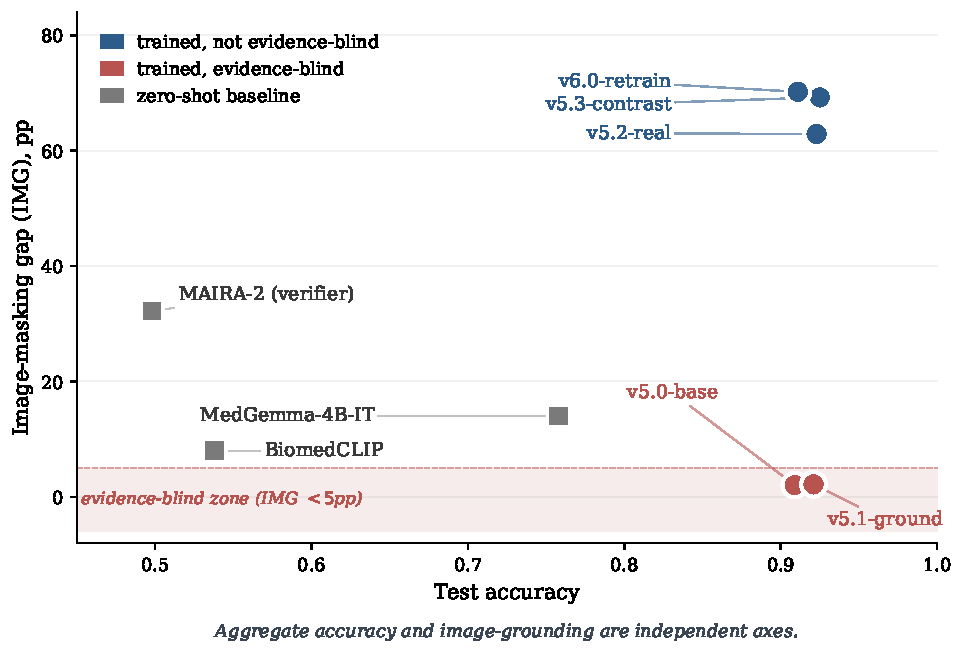
\includegraphics[width=\linewidth]{figures/F2_decoupling_scatter.pdf}
\caption{\textbf{Aggregate accuracy and image-grounding are independent
axes.} Circles: trained configurations. Squares: zero-shot detectors on
a $500$-claim real-RRG subset. Shaded band: evidence-blind zone
($\mathrm{IMG} < 5$\,pp). The highest-validation-accuracy configurations
(v5.0, v5.1) sit in the blind zone at $90$--$92\%$ accuracy; zero-shot
baselines BiomedCLIP and MedGemma-4B-IT are blind on the ESG axis at
intermediate accuracy.}
\label{fig:decoupling}
\end{figure}

\paragraph{Field audit on real-RRG hallucinations.} We extend the
diagnostic to $500$ silver-labelled real-RRG claims with four zero-shot
detectors (Fig.~\ref{fig:decoupling}; full numbers in
Appendix~\ref{app:fieldaudit}). BiomedCLIP zero-shot reaches $0.538$
accuracy with IMG $= 8.0$\,pp and ESG $= 0.0$\,pp (blind on ESG).
MedGemma-4B-IT used as a verifier reaches $0.758$ with IMG $= 14.0$\,pp
and ESG $= 2.0$\,pp (blind on ESG). MAIRA-2 used zero-shot clears both
thresholds (IMG $= 32.2$\,pp, ESG $= 6.6$\,pp) but at near-chance
accuracy ($0.498$). The combination matters: a verifier can fail one
axis without failing the other, and aggregate accuracy alone does not
predict the joint outcome.

\paragraph{Cross-site regression and deployment alarm.} Two leave-one-
site-out configurations trained under the v5.3 loss composition show the
mitigation does not transfer (Table~\ref{tab:headline}, bottom). Held-
out OpenI regresses to IMG $= 3.21$\,pp (within $1.2$\,pp of the v5.0
baseline); held-out ChestX-Det10 keeps most of the IMG mitigation but
drops to ESG $= 2.69$\,pp, below threshold. \emph{The same three metrics
that catch training-time blindness catch post-deployment blindness.}
This is the second role of the same diagnostic.

\paragraph{Conformal selection collapses on blind verifiers.} We wrap an
inverted conformal Benjamini--Hochberg procedure around each verifier's
support score, calibrated on a held-out $4{,}046$-claim calibration
split at target $\alpha = 0.10$. Only v5.3-contrast produces a populated
trusted set: $n_{\mathrm{green}} = 985$ claims with achieved
$\mathrm{FDR} = 0.91\%$ and power $39.6\%$. The configurations v5.0,
v5.1, and v5.2 collapse to $n_{\mathrm{green}} = 0$; v5.0 and v5.1
collapse because they are evidence-blind, and v5.2 collapses because the
joint distribution of (support score, true label) is not separable
enough below the target level (Appendix~\ref{app:conformal}). A
conformal guarantee on a blind verifier has nothing to certify.

\section{Discussion}
\label{sec:discussion}

The cross-entropy baseline reports a competitive $90.9\%$ test accuracy
while being image-blind at IMG $= 2.03$\,pp. The consistency loss and HO
filter act on disjoint failure modes: the consistency loss penalises
verdict-invariance under image masking, and the HO filter downweights
training rows the text-only model already solves. Adding patch
grounding alone (v5.1) does not move IMG, mirroring NLI partial-input
findings \citep{gururangan2018annotation, poliak2018hypothesis} that
auxiliary supervision on input attribution does not by itself prevent
shortcut exploitation.

\emph{The mitigation indexes on training-distribution shortcuts.} Under
$\mathrm{site}_{\mathrm{train}} \neq \mathrm{site}_{\mathrm{test}}$, the
shortcut structure changes and the mitigation has nothing to suppress
--- but the same diagnostic catches the post-shift blindness. This
makes the counterfactual diagnostic the appropriate alarm signal in
both training-time selection and deployment-time monitoring; the
appropriate \emph{fix} for the cross-site regime is distribution-shift-
aware methodology (e.g., weighted conformal inference under covariate
shift \citep{tibshirani2019conformal}) layered on top of the same
diagnostic.

The conformal-selection collapse on blind verifiers sharpens the
Mohri--Hashimoto conformal-factuality guarantee
\citep{mohri2024conformal}: marginal coverage is preserved on whatever
signal the underlying verifier emits, but if that signal is image-blind
the resulting trusted set has no clinical content. Wrapping a frozen
verifier in conformal selection is \emph{necessary but not sufficient}
for trustworthy deployment.

\section{Limitations and Conclusion}
\label{sec:limits}

Three limitations bound our claims. \textbf{(L1) Scale.} The benchmark
spans approximately $7{,}500$ images and $25{,}176$ training claims ---
enough to expose evidence-blindness as a measurable failure mode but
not to estimate its prevalence at population scale. \textbf{(L2)
Single-seed training.} All training runs use a single random seed;
multi-seed replication is deferred to an extended version. \textbf{(L3)
Spatial residual.} Laterality-turning claims are insensitive to
horizontal flips (IPG within $[-0.88, +0.88]$\,pp across all
configurations); the consistency loss targets image \emph{presence}
rather than spatial arrangement, and closing this residual would
require an image-encoder-level intervention.

We introduced a counterfactual diagnostic for multimodal medical claim
verification (IMG, ESG, IPG), a training-time recipe that closes the
in-distribution IMG from $2.03$\,pp to $69.24$\,pp at $+1.6$\,pp
accuracy, and the empirical observation that inverted conformal
selection collapses to an empty trusted set on every evidence-blind
verifier we tested. Counterfactual evidence-sensitivity testing should
precede aggregate-accuracy reporting and conformal trust-selection for
any multimodal medical verifier. Benchmark maintainers and submission
checklists in this area should report partial-input baselines alongside
aggregate accuracy --- as the NLI community did after
\citet{gururangan2018annotation} and \citet{poliak2018hypothesis}.

\bibliographystyle{icml2026}
\bibliography{pivot_ab_references}

\appendix

\section{Threshold Sensitivity for IMG and ESG}
\label{app:thresholds}

The body of the paper treats a verifier as evidence-blind if
$\mathrm{IMG} < 5$\,pp or $\mathrm{ESG} < 5$\,pp. We chose the $5$\,pp
threshold by sweeping $\{3, 5, 7, 10\}$\,pp on the validation split and
selecting the operating point that maximally separated the v5.0 / v5.1
baselines (whose IMG is $\sim 2$\,pp) from the v5.2 / v5.3 / v6.0
configurations (whose IMG is $\geq 60$\,pp). The qualitative finding
(``the highest-validation-accuracy configuration is evidence-blind'') is
robust across all four thresholds tested. ESG is informative on this
benchmark only as a coarse pass/fail signal because every trained
configuration sits in the $[18.56, 21.13]$\,pp band; this is consistent
with the dataset-dependence of partial-input gaps reported by
\citet{poliak2018hypothesis}.

\section{Training Hyperparameters}
\label{app:training}

\begin{table*}[t]
\centering
\small
\caption{Training hyperparameters shared across all reported
configurations. Per-configuration loss-weight settings are derived from
Section~\ref{sec:methods}; full per-configuration YAML is in the
released codebase.}
\begin{tabular}{ll}
\toprule
Image backbone & BiomedCLIP ViT-B/16 (top 4 of 12 blocks trainable) \\
Text backbone & RoBERTa-large (top 8 of 24 layers trainable) \\
Shared dim / fusion layers & $d = 768$, $4$ cross-modal layers, $12$ heads \\
Verdict head & 2-way softmax on a learned $[\mathrm{VERDICT}]$ token \\
Support-score head & sigmoid scalar for conformal calibration \\
Grounding head & $14 \times 14$ patch sigmoid map \\
Optimizer & AdamW \\
LR (encoders / heads) & $1\times 10^{-5}$ / $5\times 10^{-5}$ \\
Weight decay & $0.01$ \\
Warm-up / schedule & $500$-step linear warm-up, cosine decay to zero \\
Batch size / grad accum & $32$ / $2$ \\
Precision & bf16 \\
HO-filter activation threshold & $0.7$ on $p_{\text{text}}^{\text{correct}}$ \\
HO-filter $\mathcal{L}_{\mathrm{cls}}$ downweight & $0.2\times$ \\
$\mathcal{L}_{\mathrm{consist}}$ margin & $0.2$ \\
$\mathcal{L}_{\mathrm{contrast}}$ margin & $0.2$ \\
$\mathcal{L}_{\mathrm{uncert}}$ MC-dropout rate / samples & $0.2$ / $5$ \\
Random seed & $42$ (global) \\
\bottomrule
\end{tabular}
\end{table*}

The full composite loss is
\begin{equation*}
\mathcal{L} = \lambda_{\mathrm{cls}}\mathcal{L}_{\mathrm{cls}}
              + \lambda_{\mathrm{ground}}\mathcal{L}_{\mathrm{ground}}
              + \lambda_{\mathrm{consist}}\mathcal{L}_{\mathrm{consist}}
              + \lambda_{\mathrm{contrast}}\mathcal{L}_{\mathrm{contrast}}
              + \lambda_{\mathrm{uncert}}\mathcal{L}_{\mathrm{uncert}}
\end{equation*}
with $\lambda_{\mathrm{cls}} = 1.0$, $\lambda_{\mathrm{ground}} = 0.5$,
$\lambda_{\mathrm{consist}} = 0.3$, $\lambda_{\mathrm{contrast}} = 0.3$,
$\lambda_{\mathrm{uncert}} = 0.1$.

\section{Loss-Drop Ablations}
\label{app:ablations}

We hold the v5.3 configuration fixed and remove one loss term at a time
to identify the load-bearing components. Table~\ref{tab:ablations}
reports IMG at the resulting test-time test split.

\begin{table*}[t]
\centering
\small
\caption{Single-component drop ablations on the v5.3 configuration. IMG
collapses below the $5$\,pp evidence-blind threshold when either
$\mathcal{L}_{\mathrm{consist}}$ or the HO filter is removed; removing
the grounding, contrastive, or uncertainty terms each changes IMG by
$< 5$\,pp.}
\label{tab:ablations}
\begin{tabular}{lr}
\toprule
\textbf{Variant of v5.3} & \textbf{IMG (pp)} \\
\midrule
Full v5.3 & $69.24$ \\
$-\mathcal{L}_{\mathrm{consist}}$ (\emph{load-bearing}) & $\phantom{0}2.13$ \\
$-$ HO filter (\emph{load-bearing}) & $\phantom{0}5.85$ \\
$-\mathcal{L}_{\mathrm{ground}}$ & $66.10$ \\
$-\mathcal{L}_{\mathrm{contrast}}$ & $63.28$ \\
$-\mathcal{L}_{\mathrm{uncert}}$ & $73.40$ \\
\bottomrule
\end{tabular}
\end{table*}

The two interventions act on disjoint failure modes: the consistency
loss penalises verdict-invariance under image masking (a per-example
signal), and the HO filter downweights training rows the text-only model
already solves (a row-reweighting signal). Both are required.

\section{Benchmark Cohort and Silver-Label Protocol}
\label{app:benchmark}

\paragraph{Training cohort.} \textsc{GroundBench-v6}
aggregates three public sources: OpenI \citep{demner2016openi} (US
frontal radiographs with paired CheXbert-format reports), ChestX-Det10
\citep{liu2020chestxdet} (US radiographs with pixel annotations over
ten finding categories), and PadChest-GR \citep{castro2024padchestgr}
(bilingual Spanish/English studies with per-sentence radiologist
bounding boxes). Patient-stratified splits at $70/10/10/10$ via
MD5-hash bucketing on the patient identifier yield $28{,}361$ training,
$4{,}046$ validation, $4{,}046$ calibration, and $4{,}132$ test claims
after filtering for resolved \textsc{sup}/\textsc{con} labels.

\paragraph{Real-RRG silver labels.} For real-hallucination evaluation we
generate findings-section reports from $500$ held-out OpenI studies
using MAIRA-2 \citep{bannur2024maira2}, CheXagent-2-3B
\citep{chen2024chexagent}, and MedGemma-4B-IT \citep{google2024medgemma}.
Each generated report is decomposed into atomic claims; the three
generators yield $2{,}707$ atomic claims after decomposition. We
silver-label each claim with a three-LLM ensemble (a MIMIC-fine-tuned
grader plus two MIMIC-free graders for leakage decoupling
\citep{ostmeier2024green}) and report two-of-three majority labels.
$1{,}599$ claims resolve to \textsc{sup}, $335$ to \textsc{con}, and
$773$ to \textsc{uncertain}.

\section{Field Audit: Per-Detector Numbers}
\label{app:fieldaudit}

\begin{table*}[t]
\centering
\small
\caption{Zero-shot detectors on the $500$-claim real-RRG subset. RadFlag
is a hallucination flagger that emits a binary stability score and is
not input-conditioned; IMG/ESG do not apply (\textsc{n/a}).}
\label{tab:baselines}
\begin{tabular}{lcccc}
\toprule
\textbf{Detector} & \textbf{Acc} & \textbf{IMG (pp)} & \textbf{ESG (pp)} & \textbf{Blind?} \\
\midrule
BiomedCLIP (zero-shot)              & $0.538$ & $\phantom{0}8.0$  & $\phantom{0}0.0$  & yes \\
MedGemma-4B-IT (as verifier)        & $0.758$ & $14.0$ & $\phantom{0}2.0$  & yes \\
MAIRA-2 (as verifier)               & $0.498$ & $32.2$ & $\phantom{0}6.6$  & no  \\
RadFlag (MAIRA-2, $K{=}6$)          & $0.664$ & \textsc{n/a}  & \textsc{n/a}  & \textsc{n/a} \\
Ours (v6.0-retrain)                 & $0.911$ & $70.21$ & $20.01$ & no  \\
\bottomrule
\end{tabular}
\end{table*}

The combination of axes matters: a verifier can fail one axis without
failing the other, and aggregate accuracy alone does not predict the
joint outcome.

\section{Inverted Conformal Selection Procedure}
\label{app:conformal}

We wrap each trained verifier in an inverted conformal Benjamini--
Hochberg selection procedure calibrated against the support-score
distribution of \textsc{con} claims on a held-out $4{,}046$-claim
calibration split. The procedure follows the conformal-factuality
template of \citet{mohri2024conformal} and the FDR-controlled selection
template of \citet{gui2024conformal}. At target $\alpha = 0.10$, only
v5.3-contrast produces a non-empty trusted set: $n_{\mathrm{green}} =
985$ claims at achieved $\mathrm{FDR} = 0.91\%$ and power $39.6\%$. The
v5.0, v5.1, and v5.2 configurations collapse to $n_{\mathrm{green}} =
0$.

The mechanism is joint-distribution-driven rather than marginal:
the support-score distributions of v5.0 and v5.1 are not less sharp
than v5.3 on the marginal axis, but they fail to separate \textsc{sup}
from \textsc{con} along the score-label joint, so the calibration set's
\textsc{con} scores cover the test set densely and Benjamini--Hochberg
finds no cutoff at $\alpha = 0.10$. This is the empirical statement of
the discussion-section claim that ``conformal selection on an
evidence-blind verifier has nothing to certify.''

\section{Reproducibility Checklist}
\label{app:repro}

\textbf{Met:} (i) Training data sources are public (OpenI, ChestX-Det10,
PadChest-GR); MIMIC-CXR is not used. (ii) Patient-stratified
$70/10/10/10$ splits via MD5-hash bucketing on patient identifier. (iii)
Hyperparameters in Appendix~\ref{app:training}; per-configuration YAML
in the released codebase. (iv) Modal H100 80\,GB; bf16 mixed precision.

\textbf{Deferred to extended version:} model and code release URLs
(anonymized for double-blind review, filled at camera-ready); multi-seed
replication; PadChest-GR claim-extraction for full three-site training.

\end{document}
